\documentclass{standalone}
\usepackage{tikz}
\usetikzlibrary{patterns, positioning}


\begin{document}
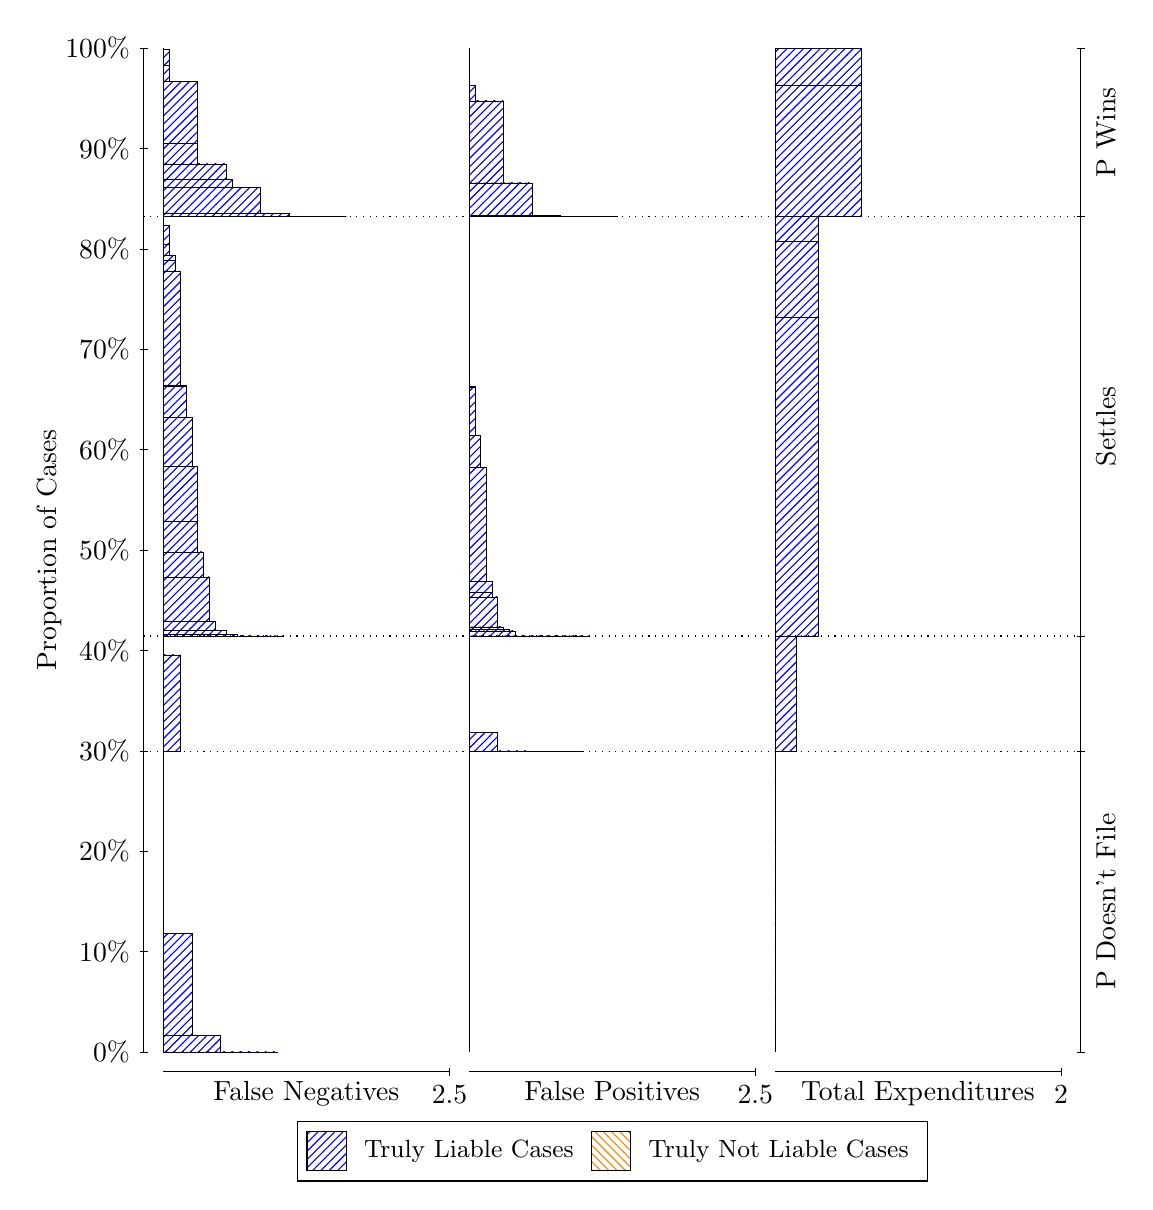
\begin{tikzpicture}
\draw[black, very thin] (1.5,1.75) -- (1.5,14.5);
\node[rotate=90, text=black, anchor=center] at (0.3, 8.125) {Proportion of Cases};
\draw[black, very thin] (1.45,1.75) -- (1.55,1.75);
\node[text=black, anchor=east] at (1.45, 1.75) {0\%};
\draw[black, very thin] (1.45,3.025) -- (1.55,3.025);
\node[text=black, anchor=east] at (1.45, 3.025) {10\%};
\draw[black, very thin] (1.45,4.3) -- (1.55,4.3);
\node[text=black, anchor=east] at (1.45, 4.3) {20\%};
\draw[black, very thin] (1.45,5.575) -- (1.55,5.575);
\node[text=black, anchor=east] at (1.45, 5.575) {30\%};
\draw[black, very thin] (1.45,6.85) -- (1.55,6.85);
\node[text=black, anchor=east] at (1.45, 6.85) {40\%};
\draw[black, very thin] (1.45,8.125) -- (1.55,8.125);
\node[text=black, anchor=east] at (1.45, 8.125) {50\%};
\draw[black, very thin] (1.45,9.4) -- (1.55,9.4);
\node[text=black, anchor=east] at (1.45, 9.4) {60\%};
\draw[black, very thin] (1.45,10.675) -- (1.55,10.675);
\node[text=black, anchor=east] at (1.45, 10.675) {70\%};
\draw[black, very thin] (1.45,11.95) -- (1.55,11.95);
\node[text=black, anchor=east] at (1.45, 11.95) {80\%};
\draw[black, very thin] (1.45,13.225) -- (1.55,13.225);
\node[text=black, anchor=east] at (1.45, 13.225) {90\%};
\draw[black, very thin] (1.45,14.5) -- (1.55,14.5);
\node[text=black, anchor=east] at (1.45, 14.5) {100\%};

\draw[black, very thin] (13.4,1.75) -- (13.4,14.5);
\draw[black, very thin] (13.35,1.75) -- (13.45,1.75);
\node[anchor=west] at (13.35, 1.75) {};
\draw[black, very thin] (13.35,5.5706) -- (13.45,5.5706);
\node[anchor=west] at (13.35, 5.5706) {};
\draw[black, very thin] (13.35,7.0332) -- (13.45,7.0332);
\node[anchor=west] at (13.35, 7.0332) {};
\draw[black, very thin] (13.35,12.358) -- (13.45,12.358);
\node[anchor=west] at (13.35, 12.358) {};
\draw[black, very thin] (13.35,14.5) -- (13.45,14.5);
\node[anchor=west] at (13.35, 14.5) {};

\draw[black, very thin, pattern color=blue, pattern=north east lines] (1.75,1.75) rectangle (3.2033,1.75);
\draw[black, very thin, pattern color=blue, pattern=north east lines] (1.75,1.75) rectangle (2.84,1.7518);
\draw[black, very thin, pattern color=blue, pattern=north east lines] (1.75,1.7518) rectangle (2.4767,1.961);
\draw[black, very thin, pattern color=blue, pattern=north east lines] (1.75,1.961) rectangle (2.1133,3.2569);
\draw[black, very thin, pattern color=orange, pattern=north west lines] (1.75,3.2569) rectangle (1.75,3.2569);
\draw[black, very thin, pattern color=blue, pattern=north east lines] (1.75,3.2569) rectangle (1.75,5.5706);
\draw[black, very thin, pattern color=blue, pattern=north east lines] (1.75,5.5706) rectangle (1.968,6.794);
\draw[black, very thin, pattern color=orange, pattern=north west lines] (1.75,6.794) rectangle (1.75,6.794);
\draw[black, very thin, pattern color=blue, pattern=north east lines] (1.75,6.794) rectangle (1.75,7.0332);
\draw[black, very thin, pattern color=blue, pattern=north east lines] (1.75,7.0332) rectangle (3.276,7.0332);
\draw[black, very thin, pattern color=blue, pattern=north east lines] (1.75,7.0332) rectangle (3.1307,7.0332);
\draw[black, very thin, pattern color=blue, pattern=north east lines] (1.75,7.0332) rectangle (2.9853,7.0332);
\draw[black, very thin, pattern color=blue, pattern=north east lines] (1.75,7.0332) rectangle (2.9127,7.0332);
\draw[black, very thin, pattern color=blue, pattern=north east lines] (1.75,7.0332) rectangle (2.84,7.0332);
\draw[black, very thin, pattern color=blue, pattern=north east lines] (1.75,7.0332) rectangle (2.7673,7.0332);
\draw[black, very thin, pattern color=blue, pattern=north east lines] (1.75,7.0332) rectangle (2.6947,7.0525);
\draw[black, very thin, pattern color=blue, pattern=north east lines] (1.75,7.0525) rectangle (2.622,7.0534);
\draw[black, very thin, pattern color=blue, pattern=north east lines] (1.75,7.0534) rectangle (2.5493,7.1025);
\draw[black, very thin, pattern color=blue, pattern=north east lines] (1.75,7.1025) rectangle (2.4767,7.1031);
\draw[black, very thin, pattern color=blue, pattern=north east lines] (1.75,7.1031) rectangle (2.404,7.2184);
\draw[black, very thin, pattern color=blue, pattern=north east lines] (1.75,7.2184) rectangle (2.404,7.2192);
\draw[black, very thin, pattern color=blue, pattern=north east lines] (1.75,7.2192) rectangle (2.3313,7.7829);
\draw[black, very thin, pattern color=blue, pattern=north east lines] (1.75,7.7829) rectangle (2.2587,8.1018);
\draw[black, very thin, pattern color=blue, pattern=north east lines] (1.75,8.1018) rectangle (2.186,8.4876);
\draw[black, very thin, pattern color=blue, pattern=north east lines] (1.75,8.4876) rectangle (2.186,9.1867);
\draw[black, very thin, pattern color=blue, pattern=north east lines] (1.75,9.1867) rectangle (2.1133,9.8102);
\draw[black, very thin, pattern color=blue, pattern=north east lines] (1.75,9.8102) rectangle (2.0407,10.201);
\draw[black, very thin, pattern color=blue, pattern=north east lines] (1.75,10.201) rectangle (2.0407,10.216);
\draw[black, very thin, pattern color=blue, pattern=north east lines] (1.75,10.216) rectangle (1.968,11.669);
\draw[black, very thin, pattern color=blue, pattern=north east lines] (1.75,11.669) rectangle (1.8953,11.803);
\draw[black, very thin, pattern color=blue, pattern=north east lines] (1.75,11.803) rectangle (1.8953,11.863);
\draw[black, very thin, pattern color=blue, pattern=north east lines] (1.75,11.863) rectangle (1.8227,12.013);
\draw[black, very thin, pattern color=blue, pattern=north east lines] (1.75,12.013) rectangle (1.8227,12.244);
\draw[black, very thin, pattern color=blue, pattern=north east lines] (1.75,12.244) rectangle (1.75,12.244);
\draw[black, very thin, pattern color=orange, pattern=north west lines] (1.75,12.244) rectangle (1.75,12.244);
\draw[black, very thin, pattern color=blue, pattern=north east lines] (1.75,12.244) rectangle (1.75,12.358);
\draw[black, very thin, pattern color=blue, pattern=north east lines] (1.75,12.358) rectangle (4.0753,12.358);
\draw[black, very thin, pattern color=blue, pattern=north east lines] (1.75,12.358) rectangle (3.712,12.359);
\draw[black, very thin, pattern color=blue, pattern=north east lines] (1.75,12.359) rectangle (3.3487,12.403);
\draw[black, very thin, pattern color=blue, pattern=north east lines] (1.75,12.403) rectangle (3.276,12.403);
\draw[black, very thin, pattern color=blue, pattern=north east lines] (1.75,12.403) rectangle (2.9853,12.733);
\draw[black, very thin, pattern color=blue, pattern=north east lines] (1.75,12.733) rectangle (2.9127,12.733);
\draw[black, very thin, pattern color=blue, pattern=north east lines] (1.75,12.733) rectangle (2.622,12.83);
\draw[black, very thin, pattern color=blue, pattern=north east lines] (1.75,12.83) rectangle (2.5493,13.028);
\draw[black, very thin, pattern color=blue, pattern=north east lines] (1.75,13.028) rectangle (2.2587,13.028);
\draw[black, very thin, pattern color=blue, pattern=north east lines] (1.75,13.028) rectangle (2.186,13.29);
\draw[black, very thin, pattern color=blue, pattern=north east lines] (1.75,13.29) rectangle (2.186,14.072);
\draw[black, very thin, pattern color=blue, pattern=north east lines] (1.75,14.072) rectangle (1.8953,14.072);
\draw[black, very thin, pattern color=blue, pattern=north east lines] (1.75,14.072) rectangle (1.8227,14.278);
\draw[black, very thin, pattern color=blue, pattern=north east lines] (1.75,14.278) rectangle (1.8227,14.48);
\draw[black, very thin, pattern color=orange, pattern=north west lines] (1.75,14.48) rectangle (1.75,14.48);
\draw[black, very thin, pattern color=blue, pattern=north east lines] (1.75,14.48) rectangle (1.75,14.5);
\draw[black, very thin, pattern color=orange, pattern=north west lines] (5.6333,1.75) rectangle (5.6333,1.75);
\draw[black, very thin, pattern color=blue, pattern=north east lines] (5.6333,1.75) rectangle (5.6333,5.5706);
\draw[black, very thin, pattern color=orange, pattern=north west lines] (5.6333,5.5706) rectangle (7.0867,5.5706);
\draw[black, very thin, pattern color=blue, pattern=north east lines] (5.6333,5.5706) rectangle (7.0867,5.5706);
\draw[black, very thin, pattern color=blue, pattern=north east lines] (5.6333,5.5706) rectangle (6.7233,5.5706);
\draw[black, very thin, pattern color=blue, pattern=north east lines] (5.6333,5.5706) rectangle (6.36,5.5724);
\draw[black, very thin, pattern color=blue, pattern=north east lines] (5.6333,5.5724) rectangle (5.9967,5.8098);
\draw[black, very thin, pattern color=blue, pattern=north east lines] (5.6333,5.8098) rectangle (5.6333,7.0332);
\draw[black, very thin, pattern color=orange, pattern=north west lines] (5.6333,7.0332) rectangle (7.1593,7.0332);
\draw[black, very thin, pattern color=blue, pattern=north east lines] (5.6333,7.0332) rectangle (7.1593,7.0332);
\draw[black, very thin, pattern color=orange, pattern=north west lines] (5.6333,7.0332) rectangle (7.014,7.0332);
\draw[black, very thin, pattern color=blue, pattern=north east lines] (5.6333,7.0332) rectangle (7.014,7.0332);
\draw[black, very thin, pattern color=orange, pattern=north west lines] (5.6333,7.0332) rectangle (6.8687,7.0332);
\draw[black, very thin, pattern color=blue, pattern=north east lines] (5.6333,7.0332) rectangle (6.8687,7.0332);
\draw[black, very thin, pattern color=blue, pattern=north east lines] (5.6333,7.0332) rectangle (6.796,7.0332);
\draw[black, very thin, pattern color=orange, pattern=north west lines] (5.6333,7.0332) rectangle (6.7233,7.0332);
\draw[black, very thin, pattern color=blue, pattern=north east lines] (5.6333,7.0332) rectangle (6.7233,7.0332);
\draw[black, very thin, pattern color=blue, pattern=north east lines] (5.6333,7.0332) rectangle (6.6507,7.0332);
\draw[black, very thin, pattern color=orange, pattern=north west lines] (5.6333,7.0332) rectangle (6.578,7.0332);
\draw[black, very thin, pattern color=blue, pattern=north east lines] (5.6333,7.0332) rectangle (6.578,7.0332);
\draw[black, very thin, pattern color=blue, pattern=north east lines] (5.6333,7.0332) rectangle (6.5053,7.0332);
\draw[black, very thin, pattern color=blue, pattern=north east lines] (5.6333,7.0332) rectangle (6.4327,7.0333);
\draw[black, very thin, pattern color=orange, pattern=north west lines] (5.6333,7.0333) rectangle (6.4327,7.0333);
\draw[black, very thin, pattern color=blue, pattern=north east lines] (5.6333,7.0333) rectangle (6.4327,7.0333);
\draw[black, very thin, pattern color=blue, pattern=north east lines] (5.6333,7.0333) rectangle (6.36,7.0335);
\draw[black, very thin, pattern color=blue, pattern=north east lines] (5.6333,7.0335) rectangle (6.2873,7.0336);
\draw[black, very thin, pattern color=orange, pattern=north west lines] (5.6333,7.0336) rectangle (6.2873,7.0336);
\draw[black, very thin, pattern color=blue, pattern=north east lines] (5.6333,7.0336) rectangle (6.2873,7.034);
\draw[black, very thin, pattern color=blue, pattern=north east lines] (5.6333,7.034) rectangle (6.2147,7.0978);
\draw[black, very thin, pattern color=orange, pattern=north west lines] (5.6333,7.0978) rectangle (6.142,7.0978);
\draw[black, very thin, pattern color=blue, pattern=north east lines] (5.6333,7.0978) rectangle (6.142,7.1159);
\draw[black, very thin, pattern color=blue, pattern=north east lines] (5.6333,7.1159) rectangle (6.0693,7.1472);
\draw[black, very thin, pattern color=blue, pattern=north east lines] (5.6333,7.1472) rectangle (6.0693,7.1478);
\draw[black, very thin, pattern color=orange, pattern=north west lines] (5.6333,7.1478) rectangle (5.9967,7.1478);
\draw[black, very thin, pattern color=blue, pattern=north east lines] (5.6333,7.1478) rectangle (5.9967,7.5286);
\draw[black, very thin, pattern color=blue, pattern=north east lines] (5.6333,7.5286) rectangle (5.924,7.5885);
\draw[black, very thin, pattern color=blue, pattern=north east lines] (5.6333,7.5885) rectangle (5.924,7.7228);
\draw[black, very thin, pattern color=blue, pattern=north east lines] (5.6333,7.7228) rectangle (5.8513,9.1757);
\draw[black, very thin, pattern color=blue, pattern=north east lines] (5.6333,9.1757) rectangle (5.7787,9.5815);
\draw[black, very thin, pattern color=blue, pattern=north east lines] (5.6333,9.5815) rectangle (5.706,10.19);
\draw[black, very thin, pattern color=blue, pattern=north east lines] (5.6333,10.19) rectangle (5.706,10.205);
\draw[black, very thin, pattern color=blue, pattern=north east lines] (5.6333,10.205) rectangle (5.6333,12.358);
\draw[black, very thin, pattern color=orange, pattern=north west lines] (5.6333,12.358) rectangle (7.5227,12.358);
\draw[black, very thin, pattern color=blue, pattern=north east lines] (5.6333,12.358) rectangle (7.5227,12.358);
\draw[black, very thin, pattern color=orange, pattern=north west lines] (5.6333,12.358) rectangle (7.1593,12.358);
\draw[black, very thin, pattern color=blue, pattern=north east lines] (5.6333,12.358) rectangle (7.1593,12.359);
\draw[black, very thin, pattern color=orange, pattern=north west lines] (5.6333,12.359) rectangle (6.796,12.359);
\draw[black, very thin, pattern color=blue, pattern=north east lines] (5.6333,12.359) rectangle (6.796,12.378);
\draw[black, very thin, pattern color=orange, pattern=north west lines] (5.6333,12.378) rectangle (6.4327,12.378);
\draw[black, very thin, pattern color=blue, pattern=north east lines] (5.6333,12.378) rectangle (6.4327,12.786);
\draw[black, very thin, pattern color=orange, pattern=north west lines] (5.6333,12.786) rectangle (6.36,12.786);
\draw[black, very thin, pattern color=blue, pattern=north east lines] (5.6333,12.786) rectangle (6.36,12.786);
\draw[black, very thin, pattern color=blue, pattern=north east lines] (5.6333,12.786) rectangle (6.0693,13.83);
\draw[black, very thin, pattern color=orange, pattern=north west lines] (5.6333,13.83) rectangle (5.9967,13.83);
\draw[black, very thin, pattern color=blue, pattern=north east lines] (5.6333,13.83) rectangle (5.9967,13.83);
\draw[black, very thin, pattern color=blue, pattern=north east lines] (5.6333,13.83) rectangle (5.706,14.029);
\draw[black, very thin, pattern color=orange, pattern=north west lines] (5.6333,14.029) rectangle (5.6333,14.029);
\draw[black, very thin, pattern color=blue, pattern=north east lines] (5.6333,14.029) rectangle (5.6333,14.5);
\draw[black, very thin, pattern color=orange, pattern=north west lines] (9.5167,1.75) rectangle (9.5167,1.75);
\draw[black, very thin, pattern color=blue, pattern=north east lines] (9.5167,1.75) rectangle (9.5167,5.5706);
\draw[black, very thin, pattern color=orange, pattern=north west lines] (9.5167,5.5706) rectangle (9.7892,5.5706);
\draw[black, very thin, pattern color=blue, pattern=north east lines] (9.5167,5.5706) rectangle (9.7892,7.0332);
\draw[black, very thin, pattern color=orange, pattern=north west lines] (9.5167,7.0332) rectangle (10.062,7.0332);
\draw[black, very thin, pattern color=blue, pattern=north east lines] (9.5167,7.0332) rectangle (10.062,11.081);
\draw[black, very thin, pattern color=orange, pattern=north west lines] (9.5167,11.081) rectangle (10.062,11.081);
\draw[black, very thin, pattern color=blue, pattern=north east lines] (9.5167,11.081) rectangle (10.062,12.041);
\draw[black, very thin, pattern color=orange, pattern=north west lines] (9.5167,12.041) rectangle (10.062,12.041);
\draw[black, very thin, pattern color=blue, pattern=north east lines] (9.5167,12.041) rectangle (10.062,12.358);
\draw[black, very thin, pattern color=orange, pattern=north west lines] (9.5167,12.358) rectangle (10.607,12.358);
\draw[black, very thin, pattern color=blue, pattern=north east lines] (9.5167,12.358) rectangle (10.607,14.029);
\draw[black, very thin, pattern color=orange, pattern=north west lines] (9.5167,14.029) rectangle (10.607,14.029);
\draw[black, very thin, pattern color=blue, pattern=north east lines] (9.5167,14.029) rectangle (10.607,14.5);
\draw[black, dotted] (1.5,5.5706) -- (13.4,5.5706);
\draw[black, dotted] (1.5,7.0332) -- (13.4,7.0332);
\draw[black, dotted] (1.5,12.358) -- (13.4,12.358);
\draw[black, very thin] (1.75,1.5) -- (5.3833,1.5);
\node[text=black, anchor=north] at (3.5667, 1.5) {False Negatives};
\draw[black, very thin] (5.3833,1.45) -- (5.3833,1.55);
\node[text=black, anchor=north] at (5.3833, 1.45) {2.5};

\draw[black, very thin] (5.6333,1.5) -- (9.2667,1.5);
\node[text=black, anchor=north] at (7.45, 1.5) {False Positives};
\draw[black, very thin] (9.2667,1.45) -- (9.2667,1.55);
\node[text=black, anchor=north] at (9.2667, 1.45) {2.5};

\draw[black, very thin] (9.5167,1.5) -- (13.15,1.5);
\node[text=black, anchor=north] at (11.333, 1.5) {Total Expenditures};
\draw[black, very thin] (13.15,1.45) -- (13.15,1.55);
\node[text=black, anchor=north] at (13.15, 1.45) {2};

\node[text=black, centered, rotate=90] at (13.72, 3.6603) {P Doesn't File};

\node[text=black, centered, rotate=90] at (13.72, 9.6959) {Settles};
\node[text=black, centered, rotate=90] at (13.72, 13.429) {P Wins};

\draw (7.449999999999999,1.5) node[draw=none] (baseCoordinate) {};
\begin{scope}[align=center]
        \matrix[scale=0.5, draw=black, below=0.5cm of baseCoordinate, nodes={draw}, column sep=0.1cm]{
            \node[rectangle, draw, minimum width=0.5cm, minimum height=0.5cm, pattern color=blue, pattern=north east lines] {}; &
            \node[draw=none, font=\small, text=black] (B) {Truly Liable Cases}; &
            \node[rectangle, draw, minimum width=0.5cm, minimum height=0.5cm, pattern color=orange, pattern=north west lines] {}; &
            \node[draw=none, font=\small, text=black] (B) {Truly Not Liable Cases}; \\
            };
\end{scope}

\end{tikzpicture}
\end{document}